%%%%%%%%%%%%%%%%%%%%%%%%%%%%%%%%%%%%%%%%%%%%%%%%%%%%%%%%%%%%%%%%%%%%%%%%%%%%%%%%
%2345678901234567890123456789012345678901234567890123456789012345678901234567890
%        1         2         3         4         5         6         7         8

\documentclass[letterpaper, 10 pt, conference]{ieeeconf}
%\documentclass[a4paper, 10pt, conference]{ieeeconf}

% This command is only needed if you want to use the \thanks command
\IEEEoverridecommandlockouts

\overrideIEEEmargins

%In case you encounter the following error:
%Error 1010 The PDF file may be corrupt (unable to open PDF file) OR
%Error 1000 An error occurred while parsing a contents stream. Unable to analyze the PDF file.
%This is a known problem with pdfLaTeX conversion filter. The file cannot be opened with acrobat reader
%Please use one of the alternatives below to circumvent this error by uncommenting one or the other
%\pdfobjcompresslevel=0
%\pdfminorversion=4

% See the \addtolength command later in the file to balance the column lengths
% on the last page of the document

% The following packages can be found on http:\\www.ctan.org
%\usepackage{graphics} % for pdf, bitmapped graphics files
%\usepackage{epsfig} % for postscript graphics files
%\usepackage{mathptmx} % assumes new font selection scheme installed
%\usepackage{times} % assumes new font selection scheme installed
%\usepackage{amsmath} % assumes amsmath package installed
%\usepackage{amssymb}  % assumes amsmath package installed

\usepackage{graphicx}
\graphicspath{{figures/}}
\usepackage[margin=1cm]{caption}

\usepackage{lipsum}

\title{\LARGE \bf
Jitterbug -- An Underactuated Continuous Control Benchmark
}

\author{
    J\'er\'emy Augot$^{1,2}$, Aaron J Snoswell$^{2}$ and Surya P. N. Singh$^{2}$
% <-this % stops a space
\thanks{
    $^{1}$ Ecole CentraleSup\'elec, Paris, France
}%
\thanks{
    $^{2}$The Robotics Design Lab at The University of Queensland, Brisbane, Australia
}%
}

\begin{document}

\maketitle
\thispagestyle{empty}
\pagestyle{empty}

%%%%%%%%%%%%%%%%%%%%%%%%%%%%%%%%%%%%%%%%%%%%%%%%%%%%%%%%%%%%%%%%%%%%%%%%%%%%%%%%
\begin{abstract}

\lipsum[1]

\end{abstract}

%%%%%%%%%%%%%%%%%%%%%%%%%%%%%%%%%%%%%%%%%%%%%%%%%%%%%%%%%%%%%%%%%%%%%%%%%%%%%%%%
\section{INTRODUCTION}

\lipsum[1]

\section{PRELIMINARIES}

\section{RELATED WORK}

\subsection{Reinforcement Learning}

\subsection{Deep Deterministic Policy Gradients (DDPG)}

\subsection{Advantage Actor-Critic (A2C)}

\subsection{Proximal Policy Optimization (PPO)}

\subsection{Deep Mind Control Suite}

\subsection{Under-actuated Control}

\begin{figure}[ht]
    
    \centering
    
    \begin{minipage}[b]{0.49\linewidth}
        \centering
        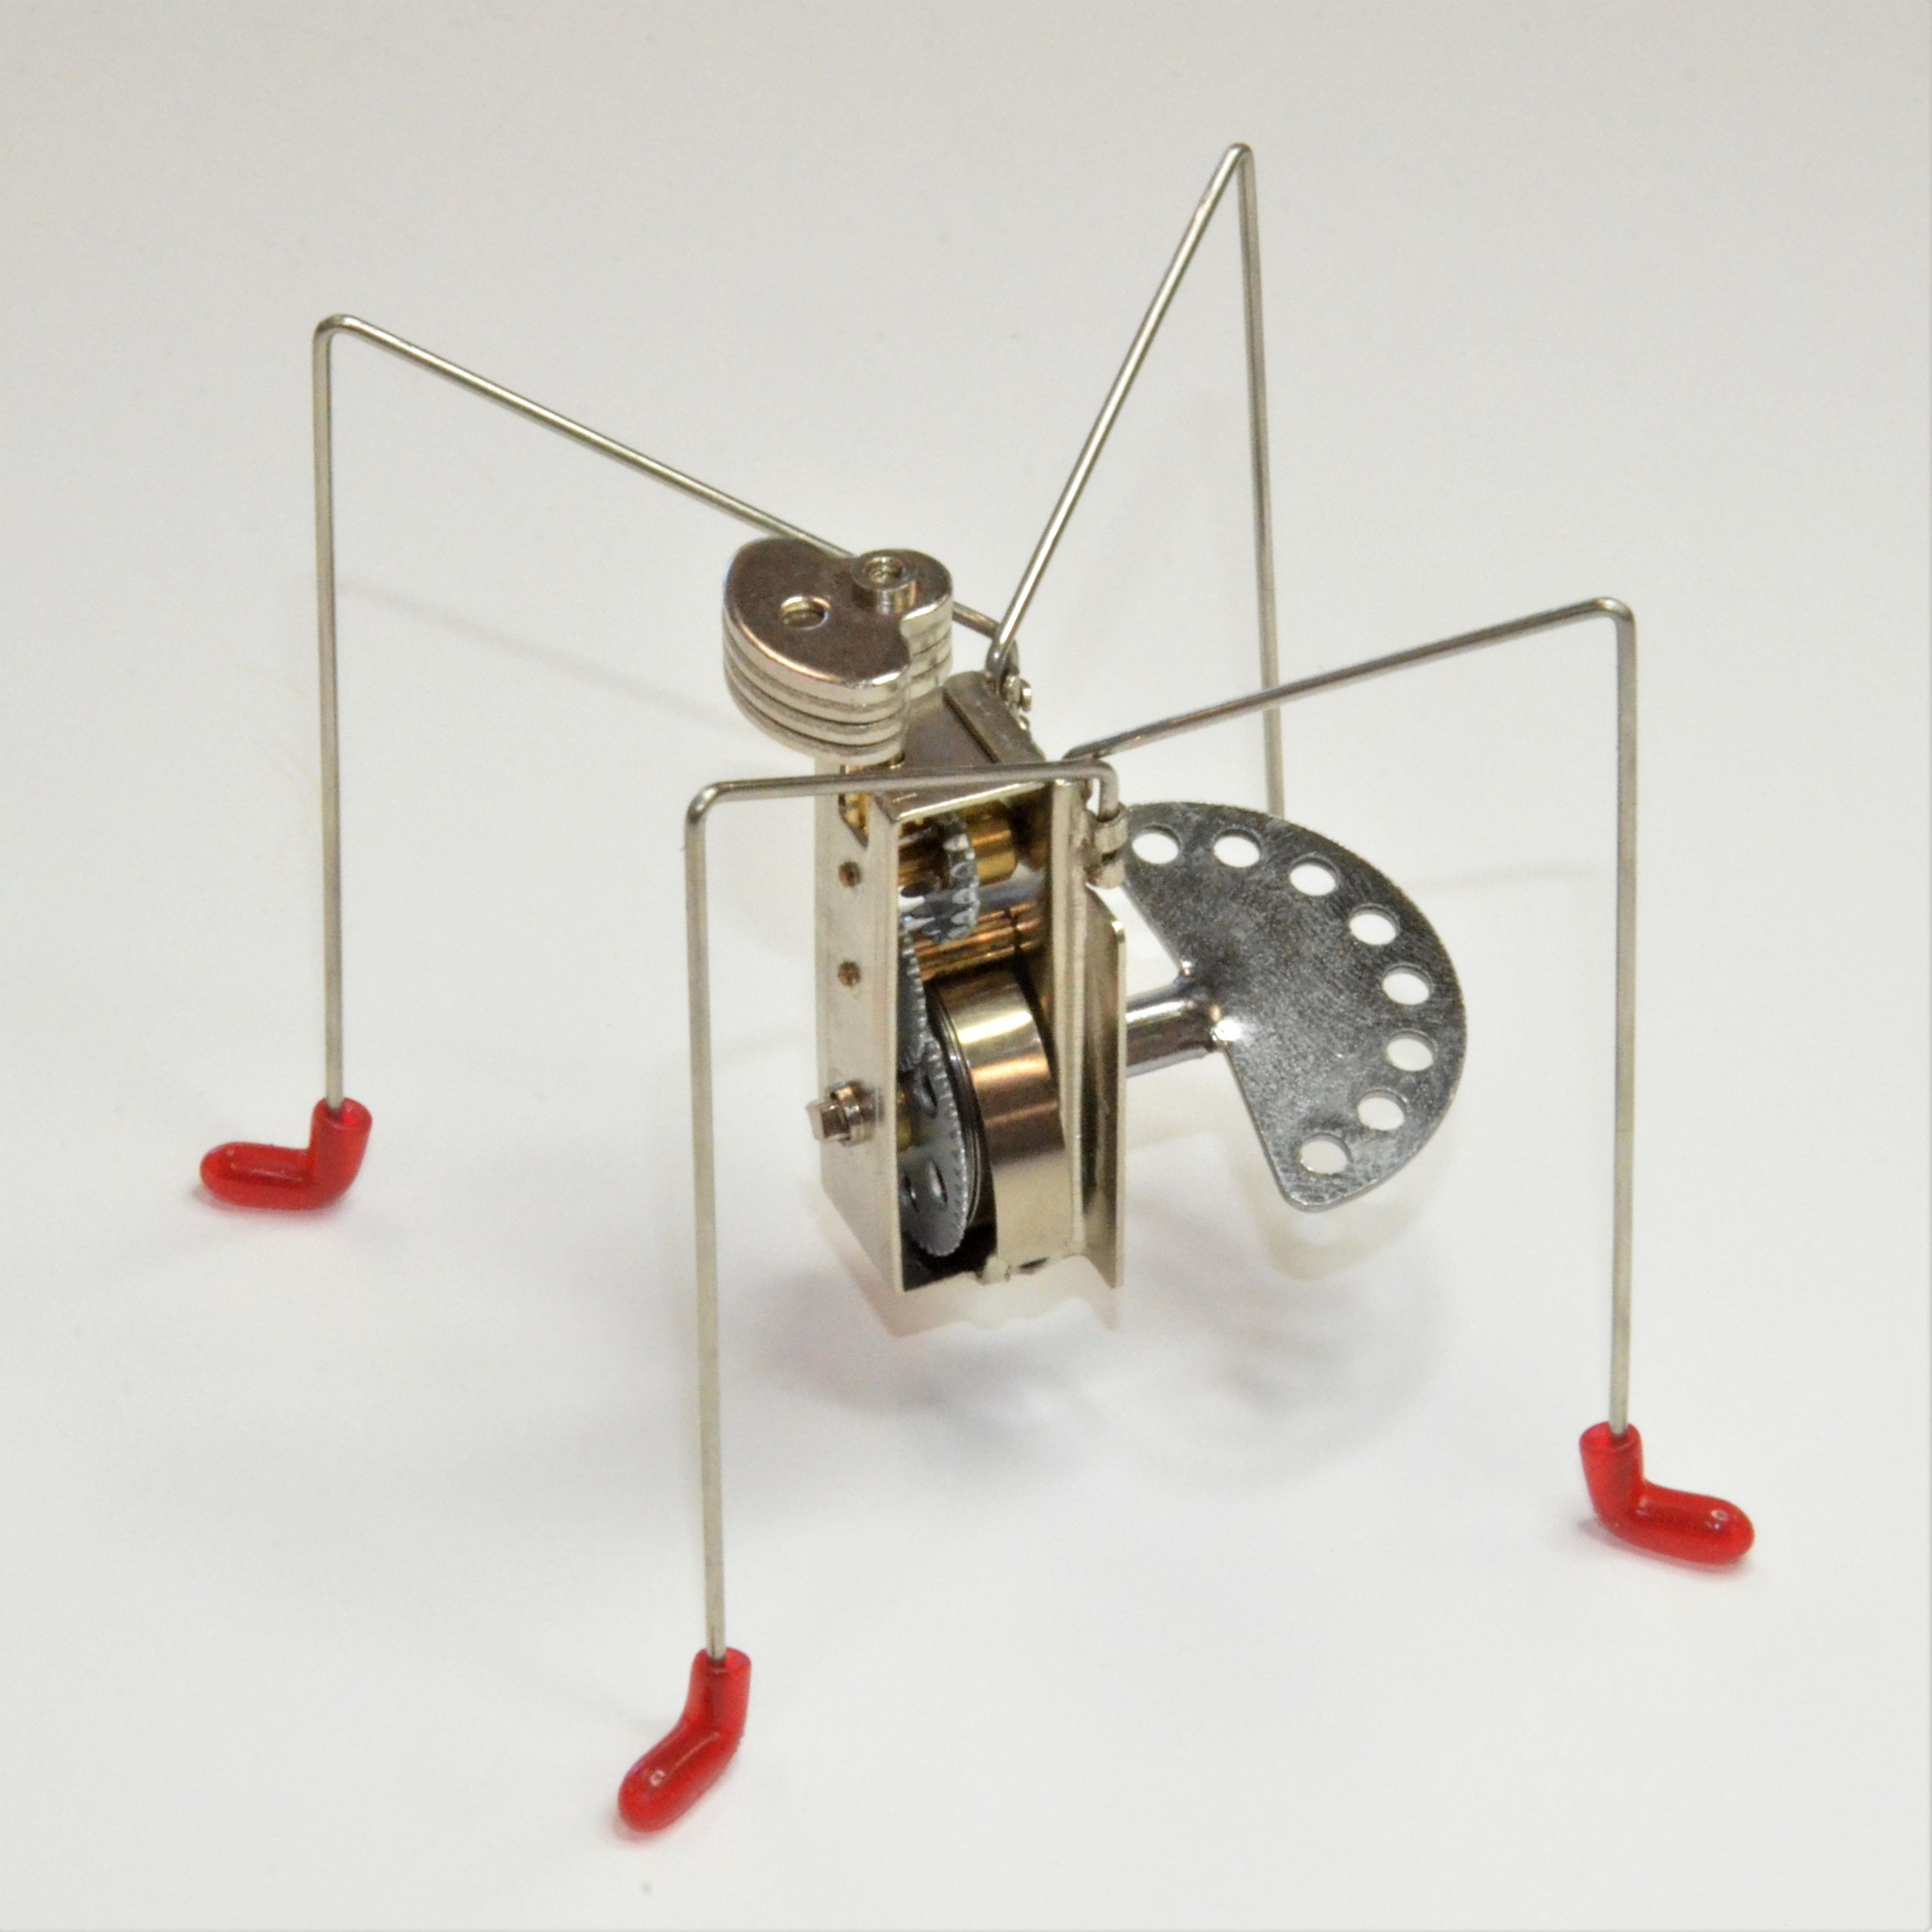
\includegraphics[width=\linewidth]{katita}
    \end{minipage}
    \begin{minipage}[b]{0.49\linewidth}
        \centering
        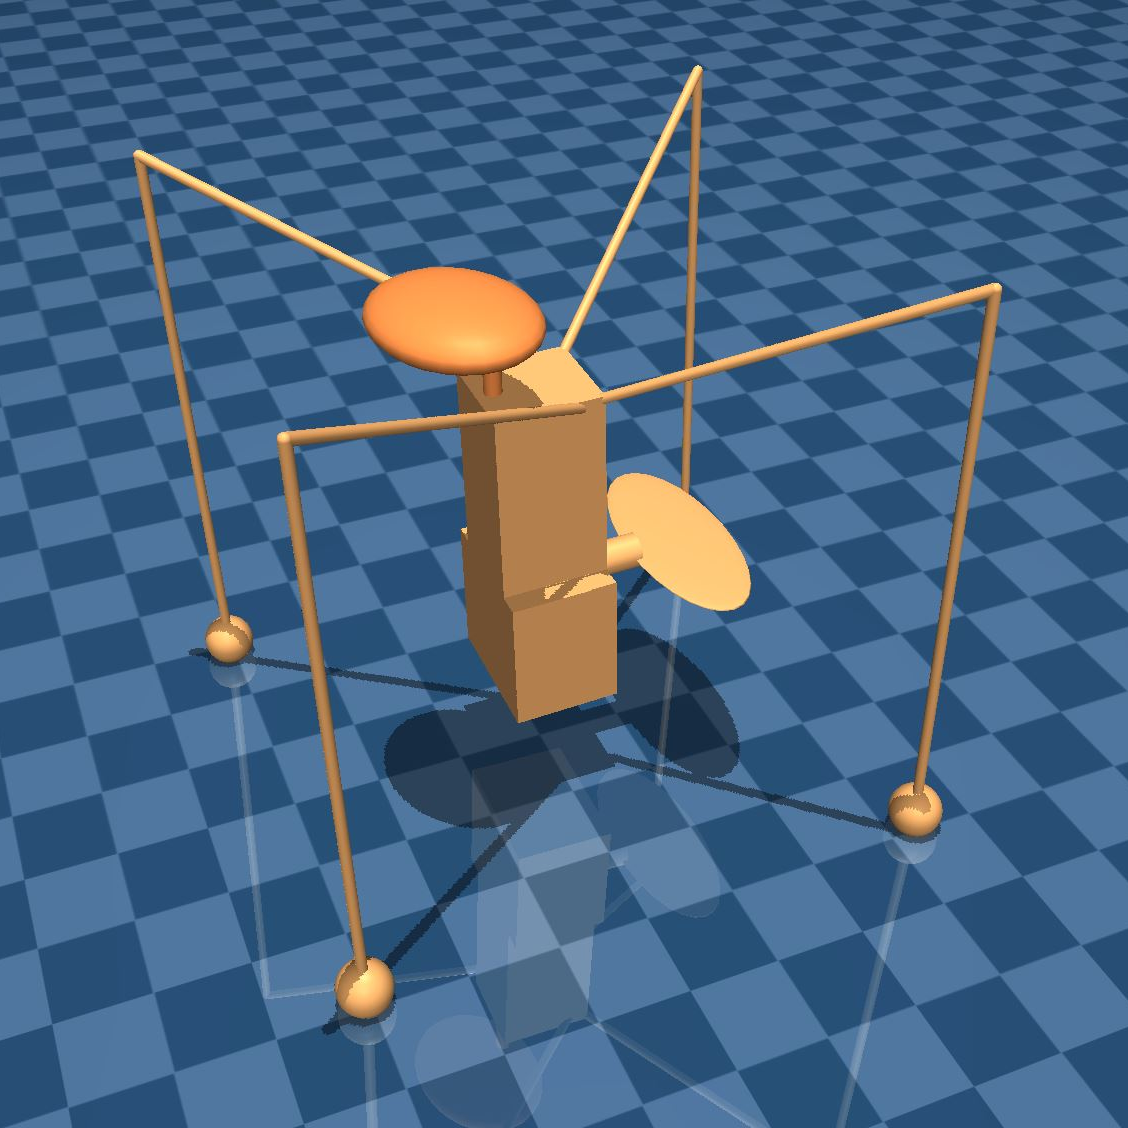
\includegraphics[width=\linewidth]{jitterbug}
    \end{minipage}
    
    \caption{
        The wind-up children's toy `Katita' (left) was the inspiration for our underactuated `Jitterbug' continuous control task (right).
        In the simulated robot the wind-up spring is replaced with a controlled single degree-of-freedom motor.
    }
    \label{fig:leader}
    
\end{figure}

\section{METHOD}

\lipsum[1]

\section{EVALUATION METRICS}

\lipsum[1]

\section{EXPERIMENTS}

\lipsum[1]

\begin{figure*}[p]
    
    \centering
    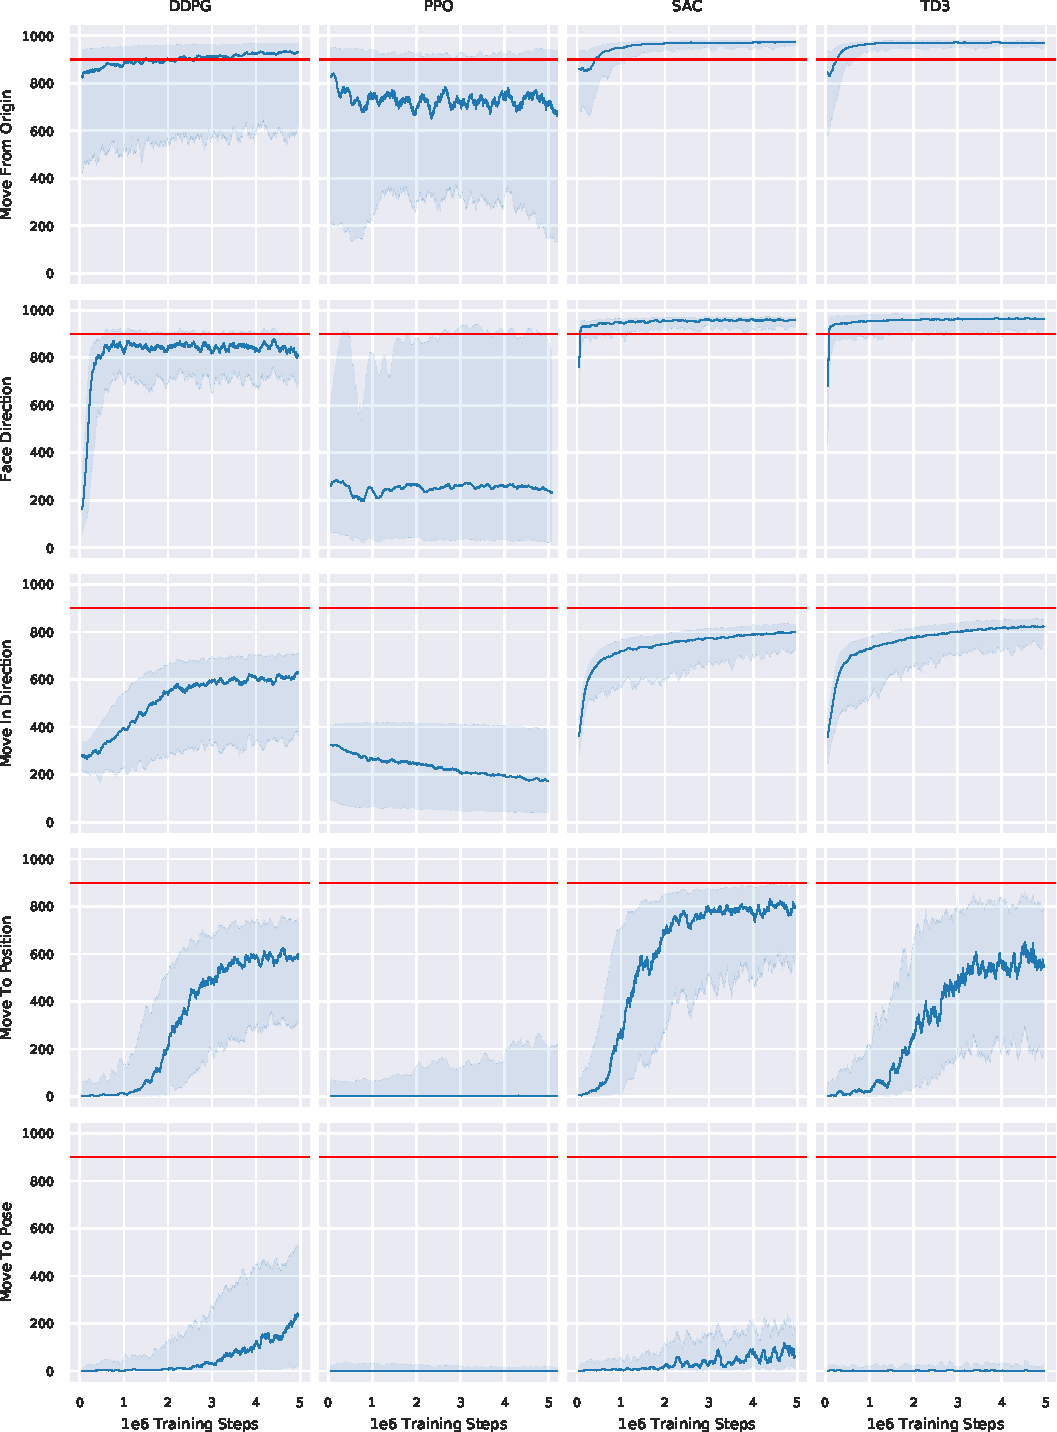
\includegraphics[width=\textwidth]{fig-rl-perf}
    
    \caption{
        Comparison of DDPG, PPO and A2C agents over environment training steps.
        We show mean and $\pm$ one standard deviation across XX random seeds in each figure.
    }
    
    \label{fig:rl-perf}
\end{figure*}

\section{CONCLUSIONS}

\lipsum[1]

%\addtolength{\textheight}{-12cm}   % This command serves to balance the column lengths
                                  % on the last page of the document manually. It shortens
                                  % the textheight of the last page by a suitable amount.
                                  % This command does not take effect until the next page
                                  % so it should come on the page before the last. Make
                                  % sure that you do not shorten the textheight too much.

%%%%%%%%%%%%%%%%%%%%%%%%%%%%%%%%%%%%%%%%%%%%%%%%%%%%%%%%%%%%%%%%%%%%%%%%%%%%%%%%



%%%%%%%%%%%%%%%%%%%%%%%%%%%%%%%%%%%%%%%%%%%%%%%%%%%%%%%%%%%%%%%%%%%%%%%%%%%%%%%%



%%%%%%%%%%%%%%%%%%%%%%%%%%%%%%%%%%%%%%%%%%%%%%%%%%%%%%%%%%%%%%%%%%%%%%%%%%%%%%%%
\section*{APPENDIX}

\lipsum[1]

\section*{ACKNOWLEDGMENT}

\lipsum[1]

%%%%%%%%%%%%%%%%%%%%%%%%%%%%%%%%%%%%%%%%%%%%%%%%%%%%%%%%%%%%%%%%%%%%%%%%%%%%%%%%

\begin{thebibliography}{99}

\bibitem{c1} G. O. Young, Synthetic structure of industrial plastics (Book style with paper title and editor), in Plastics, 2nd ed. vol. 3, J. Peters, Ed.  New York: McGraw-Hill, 1964, pp. 1564.

\end{thebibliography}


\end{document}
